\section{Juniper}

\subsection{Introduction}

Juniper Networks, Inc. is a leader of networking and security solutions in the Cloud + AI + 5G era.

While there is no Juniper equipment in Rubin's network, some of the partners of the LHN have Juniper deployments and posees extensive experience on it. 

The quotations have been made by Juniper, and can be found in the following link: \href{https://confluence.lsstcorp.org/display/IT/ITTN-043+-+Rubin+Network+Re-Engineering}{ITTN-043 Resources - Quotation}

\subsection{Hardware}

The hardware proposed by the vendor is the \href{https://www.juniper.net/us/en/products/switches/qfx-series/qfx5210-switch-datasheet.html}{QFX5210-64C-AFO2}, some of its features are:

\begin{itemize}
\item 64 x 100Gbit LAN QSFP28/QSFP+
\item Junos OS
\item 2 RU 
\item Up to 12.8 Tbps of switching throughput
\end{itemize}

\begin{figure}
    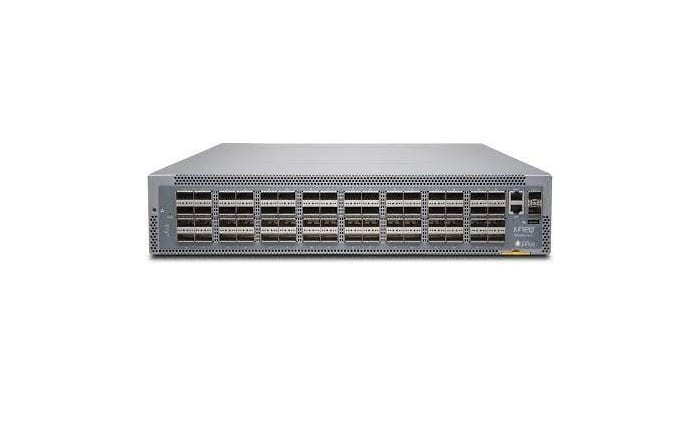
\includegraphics[width=9cm]{images/juniper_qfx5210-64c-afo2.jpeg}
    \centering
    \caption{Juniper QFX5210-64C-AFO2}
  \end{figure}


\subsection{License}

Juniper has previously sold some models of QFX series switches with the software license bundled with the physical hardware.  This practice is in the process of being discontinued and the specific SKUs for such models are being EOL’d. In general, some models of EX switch are sold with software included but modular EX chassis and QFX series chassis are sold as hardware only and a software license has to be purchased for use.

Specific to the QFX series, software options appear to be “base”, “advanced1”, “advanced2”.

See:
\begin{itemize}
\item \href{https://www.juniper.net/documentation/en_US/release-independent/licensing/topics/topic-map/software_features_that_require_licenses.html}{Software Features That Require Licenses on the QFX Series}
\item \href{https://www.juniper.net/documentation/en_US/release-independent/licensing/topics/concept/flex-licenses-for-qfx.html}{Flex Software License for QFX Series Switches}
\item \href{https://www.juniper.net/documentation/en_US/release-independent/licensing/topics/topic-map/flex-software-subscription-model.html}{Flex Software License Model Overview}
\end{itemize}

Note that models of fixed configuration EX switches that may be suitable for management and basic access would not require a separate software license

\subsection{Support}

Six levels of support or “Care” are offered.  The lowest tier provides only access to technical assistance.  All other tiers are only differentiated in terms of how quickly hardware is replaced and if white glove installation service is included. See Juniper Care Services

Note that QFX series switches appear to come with a 1 year hardware warranty when purchased new.

As Next-Day/Same-Day service to the summit is almost certainly logistically impossible and any replacement equipment coming in from outside the country will plausibly be delayed by days to weeks in customs, none of these options may not make sense for Rubin as on-site spares will be required.

“Juniper Care Core” is technical support only with no RMA.  This may be a consideration for the lowest cost possible model where the 1 year hardware warranty is relied upon for replacement and technical support is only desired for the first year.

“Juniper Care Core Plus” is the same as “Juniper Care Core” but includes factory RMA for failed hardware.


\subsection{Training}

Juniper offers a fairly wide selection of training courses both pre-scheduled instructor led and “on-demand”.  There seems to be a wide variation in the cost per person of these courses.  A brief sampling of classes found a range of \$ 950 to \$ 4,750, with most courses being towards the middle of the range.

Juniper sells “All-Access Pass”es which entitles one person to unlimited training courses for a year.  The cost for a single All-Access Pass is \$ 5,995. See \href{https://learningportal.juniper.net/juniper/user_activity_info.aspx?id=ALL-ACCESS-TRAINING-PASS-HOME}{Juniper All-Access Training Pass Overview}

\subsection{{Pros/Cons}}
\subsubsection{Pros}

\begin{itemize}
\item Juniper offers 1/yr unlimited training course passes
\item Junos has a stable CLI that has been highly consistent across different classes of devices for many years.
\item Knowledge of the junos CLI for switches is directly transferable to Juniper routers and security devices.
\item The CLI has an atomic configuration commit (and rollback) model. Junos allows configuration snippets to be edited in a flat file and then merged into the running config.
\item  Juniper equipment is widely available from main retailers.  
\item Rubin Observatory has many partner organizations, such as Ampath and NCSA, which have extension experience with Juniper equipment and can be used as a technical resource.
\item  Juniper sells some models of fixed configuration EX switches, which have the full Junos CLI, with a lifetime warranty.
\item  There is a large market for used Juniper equipment.  Most models of equipment can be purchased used for evaluation, lab use, or as a spare.  Juniper allows equipment purchased on the used to be put under a maintenance contract.  Juniper also has a certified pre-owned equipment program.
\item  Juniper allows loopback IPs to be placed in the same subnet as an SVI.
\item  Foreman has out of the box support for provisioning Juniper devices.
\end{itemize}


\subsubsection{Cons}

\begin{itemize}
\item Freebsd based instead of Linux; this means no Docker support until “Evo”.
\item Juniper is migrating from Freebsd to Linux and the new OS is called “Junos Evolved”, sometimes referred to as just “Evo”.  The plan appears to be to introduce new models, such as the QFX5130, with Evo as the only supported Junos.  Evo will not be released for existing models. There are supposedly some CLI changes in Evo.  This means that in a potential future upgrade from current generation Juniper equipment to future generation Juniper equipment, there will be an OS migration as well.  
\item Juniper still segments the market between routers and switches.
\item Junos does not allow arbitrary shell scripts to be triggered by events.
\item Rubin's network engineers does not have experience with Juniper devices.
\end{itemize}

\subsection{Closing Comments}

Juniper provides hardware with good performance running on a reliable operating system. It is also priced competitively.

There were extensive discussions with Juniper. The pre-sales support has been outstanding and we have been provided access to several internal product engineers and network architects.

The rollback feature is welcomed, however the cli interface and flow is different from Cisco devices, hence there is a learning curve for Rubin's network engineers. 

Juniper strongly embraces open standards based networking and there is a large installed base and user community around Juniper equipment.

